\documentclass{standalone}
\usepackage{tikz}

\begin{document}

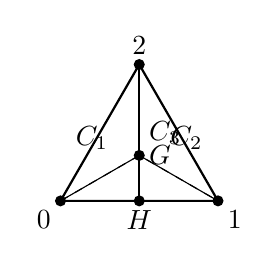
\begin{tikzpicture}
    % Define points
    \coordinate (0) at (0,0);
    \coordinate (1) at (2,0);
    \coordinate (2) at (1,{sqrt(3)});
    \coordinate (H) at (1,0);
    \coordinate (G) at (1,{sqrt(3)/3});

    % Draw triangle
    \draw[thick] (0) -- (1) -- (2) -- cycle;
    
    % Draw medians
    \draw[dashed] (0) -- (G) -- (1);
    \draw[dashed] (2) -- (G) -- (H);

    % Draw height
    \draw[thick] (2) -- (H);
    
    % Draw inner lines
    \draw (0) -- (G);
    \draw (1) -- (G);

    % Dots at points
    \foreach \p in {0, 1, 2, H, G} {
        \fill[black] (\p) circle (2pt);
    }

    % Label points
    \node[below left] at (0) {$0$};
    \node[below right] at (1) {$1$};
    \node[above] at (2) {$2$};
    \node[below] at (H) {$H$};
    \node[right] at (G) {$G$};

    % Label segments
    \node at (0.4,0.8) {$C_1$};
    \node at (1.6,0.8) {$C_2$};
    \node[right] at (1,{sqrt(3)/2}) {$C_3$};

\end{tikzpicture}

\end{document}